\documentclass{beamer}
\usetheme{ConnectivityLab}
\usepackage{times}
\usepackage{graphicx}
\usepackage{verbatim}
\usepackage{outlines}
\usepackage{fancyhdr}
\usepackage{subfigure}
\usepackage{cancel}
\usepackage{bibentry}
\usepackage{varwidth}
\usepackage{etoolbox}
\usepackage{epstopdf}

%%%%%%%%%%%%%%%%%%%%%%%%%%%%%%%%%%%%%%%%%%%%%%%%%%%%%%
%%%%%%%%%%%%%%%%%%%%%%%%%%%%%%%%%%%%%%%%%%%%%%%%%%%%%%

\title {
    Design of Privacy-Preserving Fog-assist Mobile Crowd Sensing Architecture with Ring Signature
}
\author {
    Yin-Hong Hsu
}
\date {
    05 10, 2018
}

%%%%%%%%%%%%%%%%%%%%%%%%%%%%%%%%%%%%%%%%%%%%%%%%%%%%%%
%%%%%%%%%%%%%%%%%%%%%%%%%%%%%%%%%%%%%%%%%%%%%%%%%%%%%%

\begin{document}
\begin{frame}
    \titlepage
\end{frame}

%%%%%%%%%%%%%%%%%%%%%%%%%%%%%%%%%%%%%%%%%%%%%%%%%%%%%%
%%%%%%%%%%%%%%%%%%%%%%%%%%%%%%%%%%%%%%%%%%%%%%%%%%%%%%

\begin{frame}{Zero-knowledge Proof (ZKP)}
    \begin{itemize}
        \item {The Prover proves it hold the same secure message with the Verifier.}
        \item {No secure message will be revealed within the process.}
        \item {e.g. two candidates want to find out if they have the same amount of money without disclosing the exact amount.}
        \item {The difference between RS and ZKP is RS reveal all message public and preserve users' privacy by ring size; ZKP does not reveal any secure information.}
    \end{itemize}
\end{frame}
\begin{frame}{Outline}
    \tableofcontentsgather
    \tableofcontents
\end{frame}
\section{Introduction}
\begin{frame}{Motivation}
    \begin{itemize}
        \item {In recent year, people are more focus on data monitoring and analysis.}
        \item {Also, more and more peripheral products for mobile phone and devices have become ubiquitous.}
        \item {It makes Mobile Crowd Sensing (MCS)\cite{Guo14} service more prosperity and flourish.}
        \item {How to preserve user's privacy and data correctness is the fundamental issue in MCS.}
    \end{itemize}
\end{frame}
\begin{frame}{Mobile Crowd Sensing}
    \begin{itemize}
        \item {A Technology about user's communication, computing, sensing data collection and processing.}
        \item {Can do further analysis with sensing data.}
        \item {Collecting data from sensors like ambient light, location and movement.}
    \end{itemize}
\end{frame}
\begin{frame}{Mobile Crowd Sensing}
    \begin{figure}[t]
        \centering
        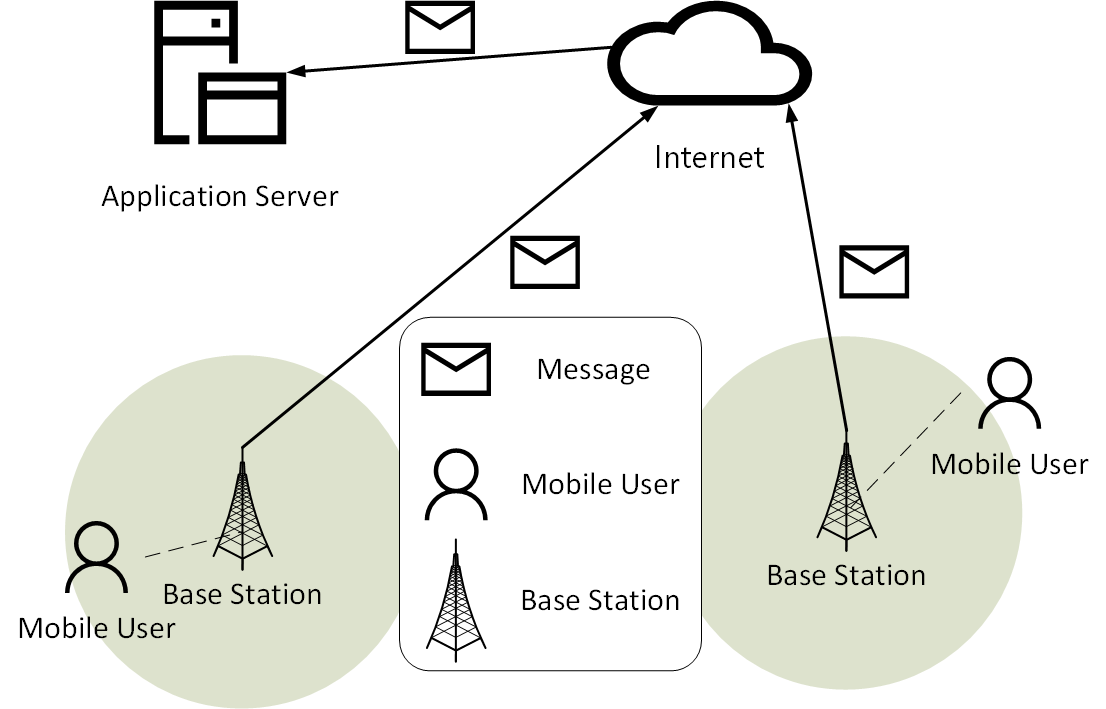
\includegraphics[width=0.8\textwidth]{figures/msc.png}
        \setbeamerfont{caption}{size=\tiny}
        \caption{Mobile Crowd Sensing}
    \end{figure}
\end{frame}
\begin{frame}{Privacy issue}
    \begin{itemize}
        \item {Fulled of privacy-sensitive information.}
        \item {Privacy information leakage might cause user location exposure and further problems.}
        \item {To provide privacy-preserving MCS service is the critical issue.}
    \end{itemize}
\end{frame}
\begin{frame}{Region-based Conditionally Anonymous Ring Signature 1/2}
    \begin{itemize}
        \item {Based on  conditionally anonymous ring signature (CARS)\cite{Zeng12}.}
        \item {The ring is built up with mobile users' identity in the region.}
        \item {The region is composed of one or multiple base station.}
        \item {Inheriting features from CARS.}
        \begin{itemize}
            \item[-] Trace
            \item[-] Revoke
        \end{itemize}
    \end{itemize}
\end{frame}
\begin{frame}{Region-based Conditionally Anonymous Ring Signature 2/2}
    \begin{itemize}
        \item {Application Server (AS) will receive numerous upload request.}
        \item {Numerous upload request cause}
        \begin{itemize}
            \item[-] Inadequate bandwidth
            \item[-] Network congestion
        \end{itemize}
        \item {Duplicated data.}
        \item {Fog-assist architecture.}
        \begin{itemize}
            \item[-] Incoming connections to AS reduced
            \item[-] Fata pre-process
        \end{itemize}
    \end{itemize}
\end{frame}
\begin{frame}{Fog computing}
    \begin{itemize}
        \item {Storage, applications, and data.}
        \item {Distributed cloud.}
        \item {Closer to end-user.}
    \end{itemize}
\end{frame}
\begin{frame}{Proposed work}
    \begin{itemize}
        \item {A Mobile Crowd Sensing (MCS) architecture.}
        \item {A privacy-preserving mechanism in MCS.}
        \item {Alleviating network congestion caused by lots of upload request.}
        \item {Deduplicated data to save bandwidth and storage.}
    \end{itemize}
\end{frame}
\begin{frame}{Illustration}
    \begin{figure}[t]
        \centering
        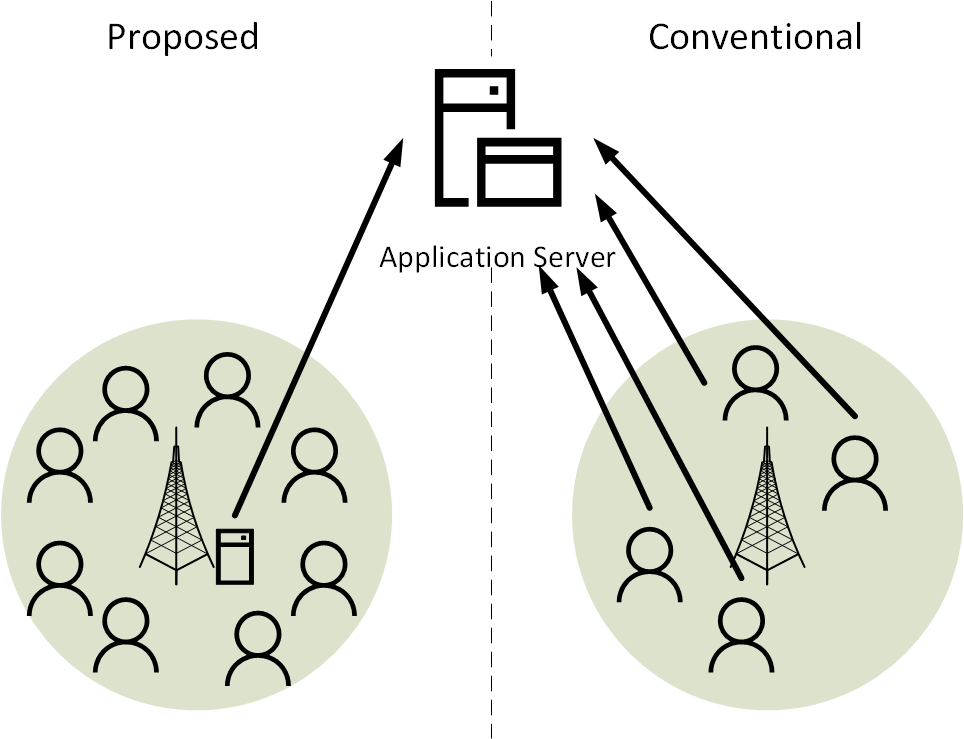
\includegraphics[width=0.8\textwidth]{figures/6.png}
        \setbeamerfont{caption}{size=\tiny}
        \caption{Comparing}
    \end{figure}
\end{frame}
%%%%%%%%%%%%%%%%%%%%%%%%%%%%%%%%%%%%%%%%%%%%%%%%%%%%%%
%%%%%%%%%%%%%%%%%%%%%%%%%%%%%%%%%%%%%%%%%%%%%%%%%%%%%%
\section{Preliminaries}
\begin{frame}{Notation}
    \begin{center}
        \begin{tabular}{ | l | l | }
            \hline
                Abbreviation                     &       Description               \\ \hline
                Param                            &       System parameter        \\ \hline
                KA                               &       Key Authority          \\ \hline
                MU                               &       Mobile User       \\ \hline
                FN                               &       Fog Node       \\ \hline
                AS                               &       Application Server       \\ \hline
                Msg                              &       Message                 \\ \hline
                $ID_{i}$                         &       Identity of $MU_{i}$           \\ \hline
                eNB                              &       eNodeB                 \\
            \hline
        \end{tabular}
    \end{center}
\end{frame}
\begin{frame}{Fog networking architecture}
    \begin{figure}[t]
        \centering
        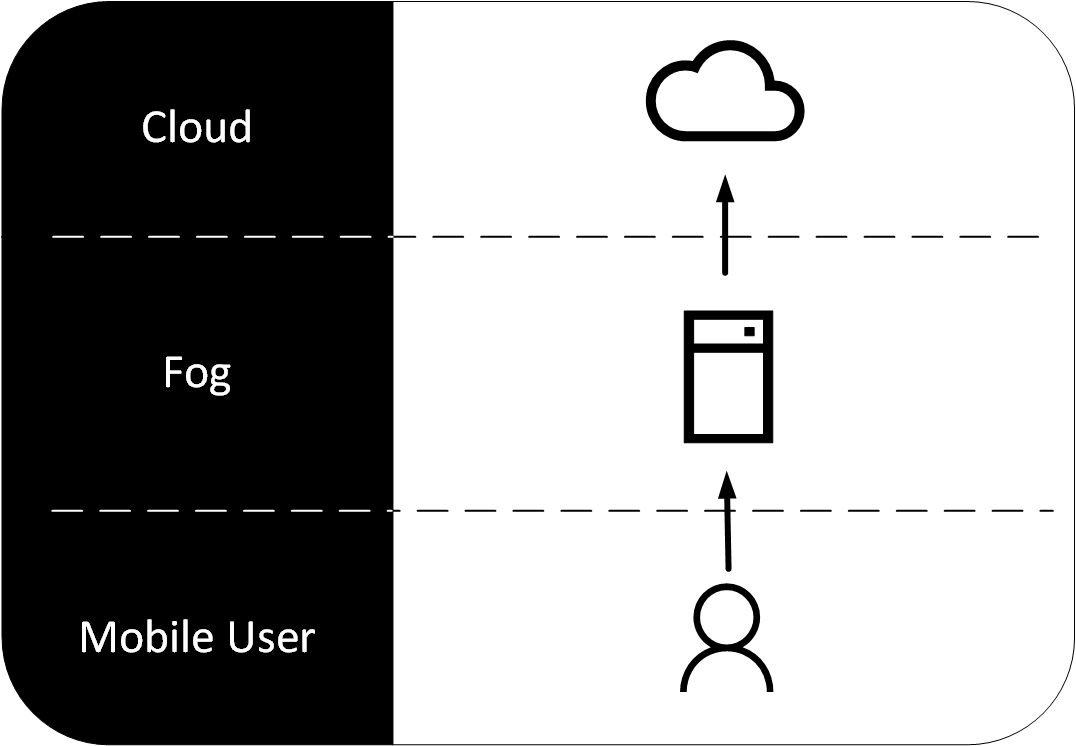
\includegraphics[width=0.8\textwidth]{figures/fog_layer.png}
        \setbeamerfont{caption}{size=\tiny}
        \caption{Fog networking architecture}
    \end{figure}
\end{frame}
\begin{frame}{Fog networking architecture 1/2}
    \begin{itemize}
        \item {Mobile device can self-organize, communicate with each other.}
        \item {Handling all communication for the near end-user.}
        \item {Fog Node act as a router, can communicate with each other.}
    \end{itemize}
\end{frame}
\begin{frame}{Fog networking architecture 2/2}
    \begin{itemize}
        \item {Reduce traffic}
        \item {Improves service quality}
        \item {Minimizes latency}
        \item {Computation capability, can alleviate computation effort from Cloud.}
    \end{itemize}
\end{frame}
% \begin{frame}{Conditionally Anonymous Ring Signature}
%     \begin{itemize}
%         \item {.}
%         \item {.}
%     \end{itemize}
% \end{frame}
%%%%%%%%%%%%%%%%%%%%%%%%%%%%%%%%%%%%%%%%%%%%%%%%%%%%%%
%%%%%%%%%%%%%%%%%%%%%%%%%%%%%%%%%%%%%%%%%%%%%%%%%%%%%%
\section{Architecture}
\begin{frame}{Architecture}
    \begin{itemize}
        \item {This framework contain 3 layers}
        \begin{itemize}
            \item[-] Cloud layer
            \item[-] Fog layer
            \item[-] Mobile user layer
        \end{itemize}
    \end{itemize}
\end{frame}
\begin{frame}{}
    \begin{figure}[t]
        \centering
        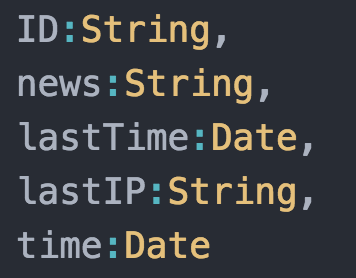
\includegraphics[width=1.0\textwidth]{figures/1.png}
        \setbeamerfont{caption}{size=\tiny}
        \caption{Architecture}
    \end{figure}
\end{frame}
\section{Procedure}
\begin{frame}{Procedure}
    \begin{itemize}
        \item {Setup and Data signing}
        % \begin{itemize}
        %     \item[-] System parameter distribution
        %     \item[-] MU key generation
        %     \item[-] MU register to the service
        %     \item[-] Signature generation
        % \end{itemize}
        \item {Data upload and pre-process}
        % \begin{itemize}
        %     \item[-] MU send signature to Fog Node
        %     \item[-] Fog Node verify the signature
        %     \item[-] Fog Node filter and aggregate data 
        %     \item[-] Send processed data to AS 
        % \end{itemize}
        \item {Mobile User Mobility and Ring Update}
        % \begin{itemize}
        %     \item[-] KA update ring to FN and MU 
        %     \item[-] Once hangover issued, the $eNB_{dest}$ will notify KA to move the public key
        % \end{itemize}
    \end{itemize}
\end{frame}
\begin{frame}{Setup}
    \begin{itemize}
        \item {This step contains parameter broadcasting, key generation, register...}
        \item {Can save bandwidth in Parameter Broadcasting and Ring Distribution step}
    \end{itemize}
\end{frame}
\begin{frame}{}
    \begin{figure}[t]
        \centering
        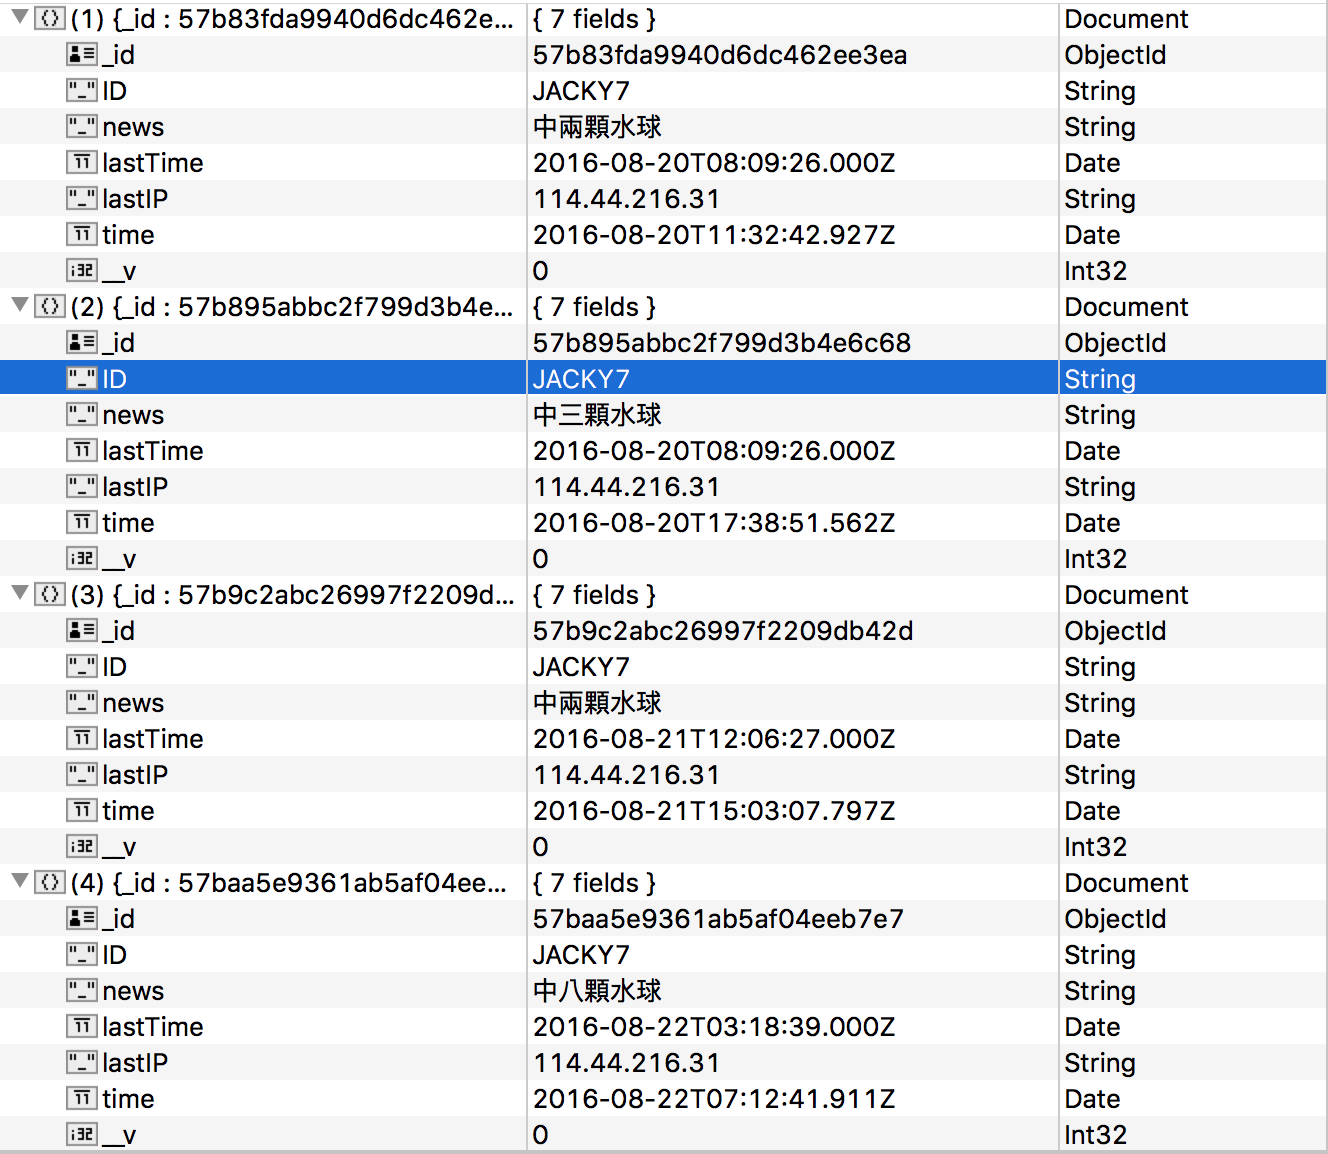
\includegraphics[width=0.6\textwidth]{figures/2.png}
        \setbeamerfont{caption}{size=\tiny}
        
    \end{figure}
\end{frame}
\begin{frame}{Data upload and pre-process}
    \begin{itemize}
        \item {Ring is in the Fog Node and MU, so the Application Server will not know the member in MCS service.}
        \item {Comparing to RCRS, the MU does not upload data directly to AS, but to the fog node and forward to AS.}
        \item {In data pre-processing step, the data will be deduplicated and structured}
    \end{itemize}
\end{frame}
\begin{frame}{}
    \begin{figure}[t]
        \centering
        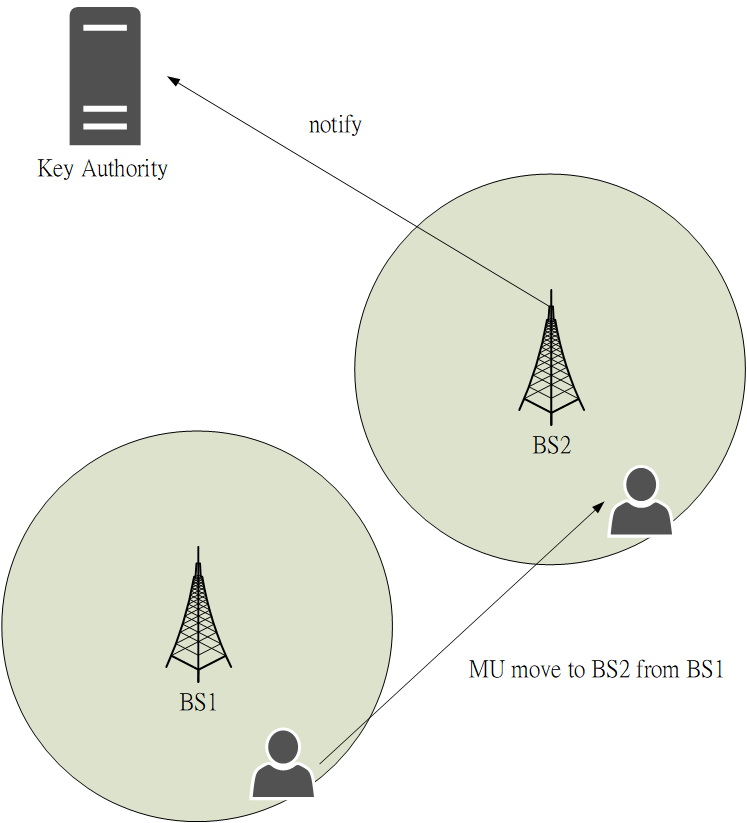
\includegraphics[width=0.6\textwidth]{figures/3.png}
        \setbeamerfont{caption}{size=\tiny}
        
    \end{figure}
\end{frame}
\begin{frame}{}
    \begin{figure}[t]
        \centering
        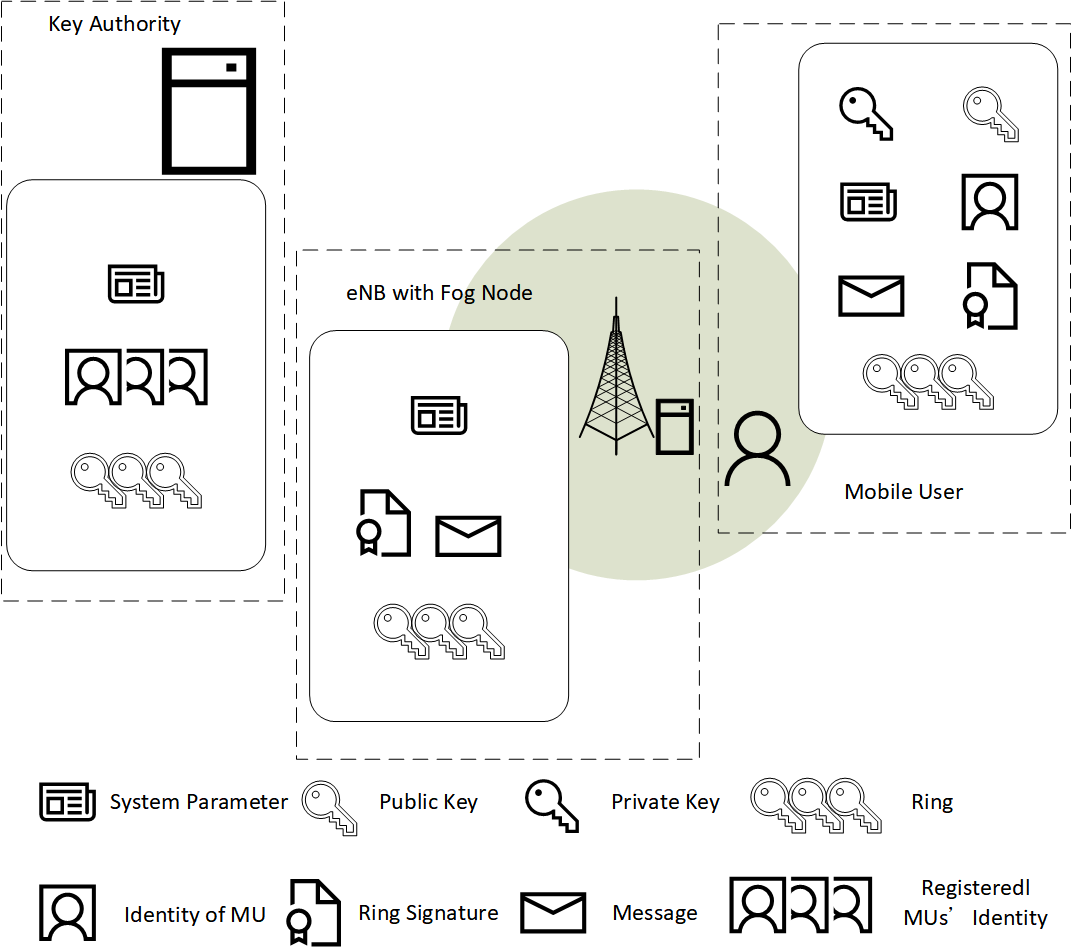
\includegraphics[width=0.8\textwidth]{figures/5.png}
        \setbeamerfont{caption}{size=\tiny}
        \caption{Data distribution}
    \end{figure}
\end{frame}
\begin{frame}{Mobile User Mobility and Ring Update}
    \begin{itemize}
        \item {When MU move to another region, the Fog Node will notify KA to move MU's public key to destination ring.}
        \item {MU only need to communicate with KA once (register).}
    \end{itemize}
\end{frame}
\begin{frame}{Mobile User Mobility and Ring Update}
    \begin{itemize}
        
        \item {KA will distribute ring to each region periodic. In RCRS, KA have to broadcast to each MU, AS; In this work, KA only have to send new rings to Fog Nodes, then each Fog Node will distribute the ring to MUs in this region.}
    \end{itemize}
\end{frame} 
\begin{frame}{}
    \begin{figure}[t]
        \centering
        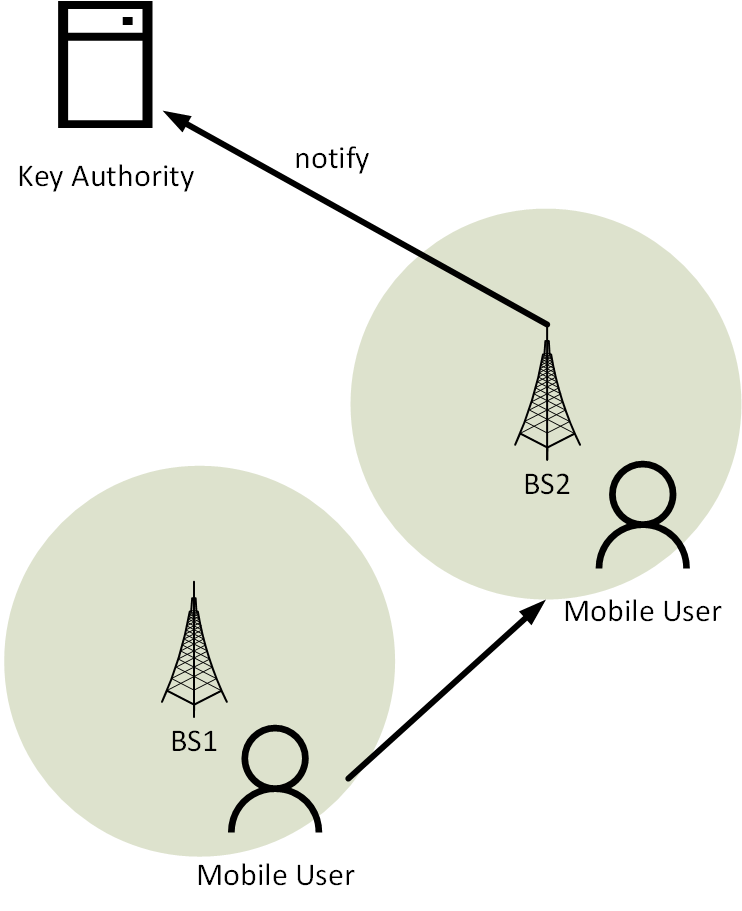
\includegraphics[width=0.6\textwidth]{figures/4.png}
        \setbeamerfont{caption}{size=\tiny}
        \caption {MU move to BS2 from BS1}
    \end{figure}
\end{frame}
\section{Attack model}
\begin{frame}{Attack model}
    \begin{itemize}
        \item {trusted:}
        \begin{itemize}
            \item[-] Key Authority
            \item[-] Fog Nodes
            \item[-] The connection between Fog Node and Fog Node
            \item[-] The connection between Fog Node and Key Authority
        \end{itemize}
        \item {untrusted:}
        \begin{itemize}
            \item[-] Mobile User
            \item[-] Application Server
            \item[-] The connection between Mobile User and Fog Node
            \item[-] The connection between Fog Node and Application Server
        \end{itemize}
    \end{itemize}
\end{frame}
\begin{frame}{Attack model}
    \begin{itemize}
        \item {Eavesdropping:}
        \begin{itemize}
            \item[-] the adversary can eavesdrop get unsafe channels to get messages. In the region-based MCS, the sensed information and the corresponding ring signatures are sent through the Internet without encryption so the adversary can get all of them
        \end{itemize}
        \item {Replay attack:}
        \begin{itemize}
            \item[-] after eavesdropping, the adversary can send a copy without modification to AS. In the RCRS, we have added a timestamp in the message structure to prevent this kind of attack so that the overdue messages would be abandoned
        \end{itemize}
    \end{itemize}
\end{frame}
\begin{frame}{Attack model}
    \begin{itemize}
        \item {Brute force:}
        \begin{itemize}
            \item[-] the adversary is able to try every possible keys and try to make the same signature as the one that matches the eavesdropped message. In the 256-bit RCRS scheme, the key space of MU’s private key contains 2 256 possible keys. It is impossible to discover the MU’s private key of the message without extremely powerful computing power
        \end{itemize}
        \item {Intersection attack:}
        \begin{itemize}
            \item[-] If a specific signer changes the ring to use every time, the adversary can easily to find out what public key the signer is actually used
        \end{itemize}
    \end{itemize}
\end{frame}
\begin{frame}{Attack model}
    \begin{itemize}
        \item {Location forgery:}
        \begin{itemize}
            \item[-] In RCRS, if the MU was compromised by adversary, the adversary can tell KA that MU is leaving to another location. So that can remove MU from current ring.
        \end{itemize}
    \end{itemize}
\end{frame}

%%%%%%%%%%%%%%%%%%%%%%%%%%%%%%%%%%%%%%%%%%%%%%%%%%%%%%
%%%%%%%%%%%%%%%%%%%%%%%%%%%%%%%%%%%%%%%%%%%%%%%%%%%%%%

\section{References}
\calcreferencespagetotal % Calc your References Page total number
\begin{frame}[allowframebreaks]{References}
    \fontsize{9pt}{13}\selectfont
    \bibliographystyle{IEEEtran}
    \bibliography{IEEEabrv,Citation}
\end{frame}

%%%%%%%%%%%%%%%%%%%%%%%%%%%%%%%%%%%%%%%%%%%%%%%%%%%%%%
%%%%%%%%%%%%%%%%%%%%%%%%%%%%%%%%%%%%%%%%%%%%%%%%%%%%%%
\section{}

\begin{frame}
    \centering
    \Large{Thanks for Your Attentions}
\end{frame}

\end{document}
